\chapter{Proportionnalité} \label{D6}

\bigskip

\begin{figure}[h]
   \centering
      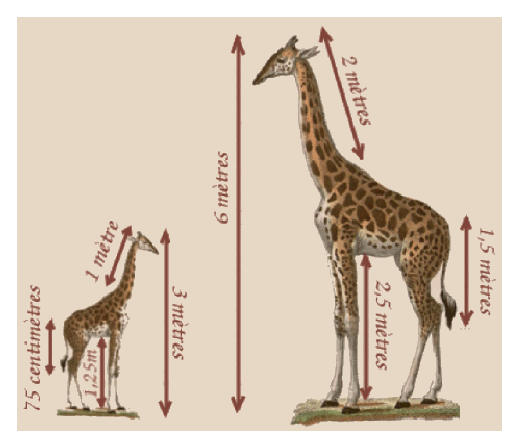
\includegraphics[height=6cm]{Organisation_gestion_donnees/Images/D6_intro_girafe}
\end{figure}

\begin{prerequis}[Un peu d'histoire] 
   La notion de proportion est présente chez {\bf Euclide} dans le {\it Livre V des Éléments} (compilation du savoirs géométriques qui resta le noyau de l'enseignement mathématique pendant près de 2\,000 ans). Voilà la définition qu'il donne de nombres proportionnels : \\
   \og{\it On dit de quatre grandeurs, $a, b, c, d$, prises dans cet ordre, que la première est à la deuxième dans le même rapport que la troisième est à la quatrième, quand n'importe quel équimultiple de la première et de la troisième grandeur est en même temps et respectivement soit supérieur, soit égal, soit inférieur à n'importe quel équimultiple de la deuxième et de la quatrième grandeur}. \fg \\
   Je laisse au lecteur le soin de traduire, en langage mathématique, cette définition ;-) \\
   Plus tard, on trouve la méthode de la {\it fausse position} : les plus anciens documents retrouvés relatifs à cette méthode remontent à une date estimée à 100 av. J.-C. dans le texte chinois intitulé {\it Les Neuf Chapitres sur l'art mathématique}.
\end{prerequis}


\cours %%%%%%%%%%%%%%%%%%%%%%%%%%%%%
%%%%%%%%%%%%%%%%%%%%%%%%%%%%%%%%

\section{Suites proportionnelles}

\subsection{Propriétés} % B

Dans toute cette section, on considère le problème suivant : {\it si 4 stylos coûtent 10 \euro, combien coûtent 12 stylos ?} \\
On considère que les stylos ont tous la même valeur afin de se trouver dans une situation de proportionnalité.

\begin{propriete}[Linéarité additive]
   Si deux suites sont proportionnelles, alors $f(x_1+x_2)=f(x_1)+f(x_2)$.
\end{propriete}

\hspace*{2cm}
\begin{minipage}{5cm}
   {\hautab{0.9}
   \begin{tabular}{|c|c|c|c|c|}
   \multicolumn{5}{l}{\setlength{\unitlength}{3ex}%
   \begin{pspicture}(4,0)(0.75,0.5) 
      \psline[linestyle=dashed,linecolor=B2]{->}(1,-0.15)(1,0.3)
      \psline[linestyle=dashed,linecolor=B2]{->}(1.8,-0.15)(1.8,0.3)
      \psline[linestyle=dashed,linecolor=B2]{->}(1,0.3)(2.6,0.3)(2.6,-0.15)
      \rput(1.4,0.05){$+$}
      \rput(2.2,0.05){$=$}
   \end{pspicture}} \\
   \hline
   4 & 5 & 9 & 18 & 6 \\
   \hline
   12 & 15 & 27 & 54 & 18 \\
   \hline
   \multicolumn{5}{l}{\setlength{\unitlength}{5ex}%
   \begin{pspicture}(4,-0.8)(0.75,0)
      \psline[linestyle=dashed,linecolor=B2]{->}(1,0.05)(1,-0.4)
      \psline[linestyle=dashed,linecolor=B2]{->}(1.8,0.05)(1.8,-0.4)
      \psline[linestyle=dashed,linecolor=B2]{->}(1,-0.4)(2.6,-0.4)(2.6,0.05)
      \rput(1.4,-0.15){$+$}
      \rput(2.2,-0.15){$=$}
   \end{pspicture}} \\
   \end{tabular}}
\end{minipage}
\begin{minipage}{8cm}
   Dans la première ligne on peut lire que $4+5 =9$. \\
   Dans la ligne du dessous, on a également $12+15 =27$.
\end{minipage}

Si 4 stylos coûtent 10 \euro{}, alors 12 stylos = 4 stylos + 4 stylos + 4 stylos coûtent 10 \euro{} + 10 \euro{} + 10 \euro{} = 30 \euro{}.

\medskip

\begin{propriete}[Linéarité multiplicative]
   Soit $k$ un réel non nul, si deux suites sont proportionnelles, alors $f(k\times x)=k\times f(x)$.
\end{propriete}

\hspace*{2cm}
\begin{minipage}{5cm}
{\hautab{0.9}
\begin{tabular}{|c|c|c|c|c|}
   \multicolumn{5}{l}{\setlength{\unitlength}{5ex}%
   \begin{pspicture}(4,0)(0.75,0.5)
      \psline[linestyle=dashed,linecolor=B2]{->}(2.5,-0.15)(2.5,0.3)(3.2,0.3)(3.2,-0.15)
      \rput(2.85,0.05){$\times2$}
      \psline[linestyle=dashed,linecolor=A1]{->}(3.35,-0.15)(3.35,0.3)(4.05,0.3)(4.05,-0.15)
      \rput(3.65,0.05){$\div3$}
   \end{pspicture}} \\
   \hline
   4 & 5 & 9 & 18 & 6 \\
   \hline
   12 & 15 & 27 & 54 & 18 \\
   \hline
   \multicolumn{5}{l}{\setlength{\unitlength}{5ex}%
   \begin{pspicture}(4,-0.8)(0.75,0)
      \psline[linestyle=dashed,linecolor=B2]{->}(2.5,0.05)(2.5,-0.4)(3.2,-0.4)(3.2,0.05)
      \rput(2.85,-0.15){$\times2$}
      \psline[linestyle=dashed,linecolor=A1]{->}(3.35,0.05)(3.35,-0.4)(4.05,-0.4)(4.05,0.05)
      \rput(3.65,-0.15){$\div3$}
   \end{pspicture}} \\
   \end{tabular}}
\end{minipage}
\begin{minipage}{8cm}
      Dans la première ligne on a $9\times2=18$ et $18\div3 =6$. \\
      Dans la ligne du dessous, $27\times2 =54$ et $54\div3 =18$.
\end{minipage}

   Si 4 stylos coûtent 10 \euro{}, alors 12 stylos = 3$\times$4 stylos coûtent 3$\times$10 \euro{} = 30 \euro{}.

\medskip

\begin{propriete}[Coefficient de proportionnalité]
Le coefficient de proportionnalité est le coefficient multiplicateur permettant de passer d'une grandeur à une autre (à ne pas confondre avec le coefficient de linéarité multiplicative).
\end{propriete}

{\psset{yunit=0.6}
\begin{pspicture}(-6,0)(9,3.5)
   \psframe(-0.5,0)(3,2)
   \psline(1,0)(1,2)
   \psline(2,0)(2,2)
   \psline(-0.5,1)(3,1)
   \rput(0.25,1.5){masse}
   \rput(0.25,0.5){prix}
   \rput(1.5,1.5){2 kg}
   \rput(1.5,0.5){3 \euro}
   \rput(2.5,1.5){4 kg}
   \rput(2.5,0.5){6 \euro}
   \psarc[linecolor=A1]{<-}(2,1.9){0.5}{20}{160}
   \rput(4.8,2.95){\textcolor{A1}{$\times2$ : coefficient de linéarité multiplicative}}
   \psarc[linecolor=B2]{<-}(3.1,1){0.35}{-90}{90}
   \rput(6.3,1){\textcolor{B2}{$\times1,5$ : coefficient de proportionnalité}}
\end{pspicture}}

Si 4 stylos coûtent 10 \euro{}, le coefficient de proportionnalité est de 2,5 car $4\times2,5 =10$. Alors, 12 stylos coûtent 30 \euro{} car $12\times2,5 =30$.

\medskip

\begin{propriete}[Produit en croix]
   Dans un tableau de proportionnalité, les produits \og en diagonale \fg{} (ou produits en croix) sont deux à deux égaux. Ceci permet de déterminer une quatrième proportionnelle.
\end{propriete}

\medskip

Pour nos stylos, on a le tableau de proportionnalité suivant : 
   \begin{tabular}{|l|C{0.8}|C{0.8}|}
      \hline
      \cellcolor{lightgray!50}nombre de stylos & 4 & 12 \\
      \hline
      \cellcolor{lightgray!50}prix des stylos en \euro & 10 & $x$ \\
      \hline
   \end{tabular}

   D'où l'égalité : $4\times x=10\times12$. \\  
   On calcule la donnée manquante : $x = \dfrac{10\times12}{4} =30$. \\
   12 stylos coûtent 30 \euro{}.

\subsection{Lien avec les fonctions linéaires} % A

\begin{definition}[Suites proportionnelles et coefficient de proportionnalité]
   Deux suites de $n$ nombres réels $(x_1,x_2,\dots,x_n)$ et $(y_1,y_2,\dots,y_n)$ sont \textbf{proportionnelles} si l'une est l'image de l'autre par une fonction linéaire $f$ définie par $y=f(x)=a\times x$ où le nombre non nul $a$ est le \textbf{coefficient de proportionnalité}.
\end{definition}

\begin{exemple}[0.5]
   On considère les suites $(\,0\,;\,1\,;\,2\,;\,3\,;\,4\,)$ et $\,0\,;\,0,5\,;\,1\,;\,1,5\,;\,2\,)$ : \\ [1mm]
   {\hautab{1.3}
   \begin{tabular}{|l|c|c|c|c|c|}
      \hline
      \cellcolor{lightgray!50} abscisse & 0 & 1 & 2 & 3 & 4 \\
      \hline
      \cellcolor{lightgray!50}ordonnée & 0 & 0,5 & 1 & 1,5 & 2 \\
      \hline
   \end{tabular}}
   $\downarrow\times0,5$ \\ [1mm] 
   Ce tableau est un tableau de proportionnalité. 
\correction
   Le coefficient de proportionnalité : $0,5$ est le coefficient directeur de la droite. \\  
   {\psset{yunit=0.55cm}
   \begin{pspicture}(-1,-1.1)(5,3)
     \psaxes{->}(5.4,2.7)
     \psline[linecolor=A1](0,0)(5,2.5)
     \psline[linestyle=dotted](1,0)(1,.5)(0,.5)
     \psline[linestyle=dotted](2,0)(2,1)(0,1)
     \psline[linestyle=dotted](3,0)(3,1.5)(0,1.5)
     \psline[linestyle=dotted](4,0)(4,2)(0,2)
   \end{pspicture}}
\end{exemple}

\begin{propriete}[Reconnaissance graphique d'une situation proportionnelle]
   On reconnaît une situation de proportionnalité lorsque le support des points représentant la situation est une droite passant par l'origine du repère.
\end{propriete}



\section{Exemples de de situations de proportionnalité classiques} % C


\subsection{Mouvement à vitesse constante} %%%%%%%

   La vitesse moyenne est caractéristique d'une situation de proportionnalité. \\ [2mm]
   \begin{tabular}{|l|c|c|c|c|}
      \hline
      Temps écoulé en s & $5$ & $8$ & $15$ & $100$ \\
      \hline
      Distance parcourue en m & $15$ & $24$ & $45$ & $300$ \\
      \hline
   \end{tabular}
   $\downarrow\times3$ \\ [2mm]
   Ce tableau est un tableau de proportionnalité de coefficient $3$ : la vitesse est de 3 mètres par seconde.

\begin{propriete}[Vitesse moyenne]
   La vitesse moyenne $v$ d'un objet qui parcourt une distance $d$ en un temps $t$ est $v=\dfrac{d}{t}$.
\end{propriete}

\medskip

La vitesse est une grandeur quotient, son unité dépend des unités de distance et de temps.

\begin{exemple*1}
   Une voiture parcourt 400 km en 5 heures, sa vitesse moyenne est de $\dfrac{\ukm{400}}{\uh{5}}$ \\
   $=80\,\mathrm{km/h} =\ukmh{80}$.
\end{exemple*1}


\subsection{Échelle sur une carte} %%%%%%%%

\begin{definition}[Échelle]
   L'\textbf{échelle} d'une carte est le coefficient de proportionnalité entre une mesure réelle et sa mesure sur la carte, ces deux mesures étant exprimées dans la même unité.
\end{definition}

\bigskip

   Une carte au 1/200 000 signifie que 1 cm sur la carte représente 200 000 cm sur le terrain, soit 2 km. \smallskip
   
   \begin{tabular}{|l|c|c|}
      \hline
       Distance carte (cm) & 1 & $x$ \\
      \hline
      Distance terrain (km) & 2 & 5 \\
      \hline
   \end{tabular}
   \; $x=\dfrac{1\times5}{2}= 2,5$ donc, 5 km sur le terrain sont représentés par 2,5 cm sur la carte.

\bigskip

\subsection{Calcul de pourcentages} %%%%%%%%%

\begin{definition}[Pourcentage]
   Le {\bf pourcentage} d'un effectif est le nombre qui aurait été proportionnellement obtenu si l'effectif avait été de 100.
\end{definition}

\medskip

\begin{propriete}[Pourcentage et coefficient multiplicateur]
   \begin{itemize}
      \item Pour calculer le pourcentage $p\,\%$ d'une quantité $n$, on effectue le calcul $\dfrac{p}{100}\times n$.
      \item Augmenter [resp. diminuer] une valeur de $p\,\%$ revient à la multiplier par $c_m =1+\dfrac{p}{100}$ \bigg[resp. $c_m =1-\dfrac{p}{100}$\bigg]. $c_m$ est appelé {\bf coefficient multiplicateur}. \\ [-6mm]
   \end{itemize}
\end{propriete}

\begin{exemple*1}
   Dans un collège, il y a 125 filles et 180 garçons. $40\,\%$ des filles et $60\,\%$ des garçons mangent à la cantine. Quel est le pourcentage d'élèves qui mangent à la cantine parmi tous les élèves du collège ? \\
   -- Nombre de filles qui mangent à la cantine : $40\,\%$ de 125 = $\dfrac{40}{100}\times125=50$. \\ [1mm]
   -- Nombre de garçons qui mangent à la cantine : $60\%$ de 180 = $\dfrac{60}{100}\times180=108$. \\
   -- Pourcentage d'élèves qui mangent à la cantine : 158 élèves sur 305 = $\dfrac{158}{305}\times 100\approx51,8$. \\ [1mm]
   Donc, le pourcentage d'élèves du collège qui mangent à la cantine est d'environ 51,8\,\%. \\ [5mm]
       On prévoit une augmentation de 18\,\% du nombre d'élèves à la rentrée prochaine. \\
         Le coefficient multiplicateur est de $1+\dfrac{18}{100} =1,18$ donc, il y aura $305\times1,18\approx 360$ élèves.         
\end{exemple*1}


\section{Le ratio} %%% 4

\begin{definition}[Ratio]
   \psset{unit=0.55,subgriddiv=0,gridlabels=0,fillstyle=solid}
   \begin{itemize}
      \item On dit que {\bf deux nombres} $a$ et $b$ sont, par exemple, dans le {\bf ratio} 3 : 4 si $\dfrac{a}{3} =\dfrac{b}{4}$. \\
      On parle de ratio \og trois pour quatre \fg. \\
      On peut modéliser ainsi : \quad 
      $\underbrace{\begin{pspicture}(0,0)(3,1.2)
                               \psframe[fillcolor=A2](0,0)(3,1)
                               \psgrid(0,0)(3,1)
                            \end{pspicture}}_a$ \!\!\!
     $\underbrace{\begin{pspicture}(3,0)(7,1.2)
                               \psframe[fillcolor=B2](3,0)(7,1)
                               \psgrid(3,0)(7,1)
                            \end{pspicture}}_b$ \\ [-2mm]
      \item On dit que {\bf trois nombres} $a$, $b$ et $c$ sont, par exemple, dans le {\bf ratio} 1 : 3 : 6 si $\dfrac{a}{1} =\dfrac{b}{3} = \dfrac{c}{6}$. \\
      On parle de ratio \og un pour trois pour six \fg. \\ [-8mm]
   \end{itemize}
\end{definition}

\smallskip

\begin{exemple*1}
   On souhaite partager 15 pièces d'or entre les pirates Seyon et Lloyd suivant le ratio 2 : 3. Cela veut dire que, à chaque fois que Seyon a 2 pièces, Lloyd en a 3.
   \begin{itemize}
      \item On calcule le nombre de parts à distribuer : 2 pour Seyon et 3  pour Lloyd, soit 5 parts.
      \item On divise la quantité de pièces à distribuer par le nombre de parts : \\
         $15\text{ pièces d'or}\div 5 =3\text{ pièces d'or}$ donc, une part vaut 3 pièces d'or.
      \item On distribue les parts : Seyon aura 2 parts soit 6 pièces d'or et Lloyd 3 parts soit 9 pièces d'or. \\ [-10mm]
   \end{itemize}
\end{exemple*1}



%%%%%%%%%%%%%%%%%%%%%%%%%%%%%%%
%%%%%%%%%%%%%%%%%%%%%%%%%%%%%%%
\activites

\begin{activite}[Groupement 1 - Exercice 1 - Partie 1 : vitesse]
   \ \\ [-16mm]
   \begin{QCM}
      Dans cette version adaptée du biathlon, les élèves ont à parcourir, en courant, 4 grands tours tracés avec des plots sur un stade comme sur la figure ci-dessous. \\
      À l'issue de chacun des 3 premiers tours, ils se présentent au pas de tir et lancent trois balles sur des cibles. S'ils atteignent 3 fois leur cible, ils n'ont pas de pénalité et repartent pour le grand tour suivant. En revanche, pour chaque lancer manqué, ils doivent effectuer un petit tour avant de repartir sur le grand tour. \\
Pour chaque élève on mesure la durée mise pour faire un parcours complet (grands tours + lancers + petits tours de pénalité le cas échéant). L'objectif est de mettre le moins de temps possible pour effectuer le parcours complet.

\begin{center}
   \includegraphics[width=16cm]{Organisation_gestion_donnees/Images/D6_ex_revue_EPS}
\end{center}

Dans cette partie, les élèves s’entraînent à la course sur le grand tour, sans effectuer de lancer de balles.
\begin{enumerate}
   \item Pour un élève de CE1, la longueur du grand tour est de 250 m.
      \begin{enumerate}
         \item On considère un élève, qui effectue les 4 tours en 10 minutes. Quelle est sa vitesse moyenne de course, en mètre par minute ?      
         \item Un autre élève a couru les 4 tours à la vitesse moyenne de 150 m/min. Déterminer sa vitesse moyenne en kilomètre par heure.
      \end{enumerate}
   \item Dans le tableau ci-dessous, les longueurs d’un grand tour pour des élèves de CM1 et de CM2 sont données, ainsi que les temps de course pour effectuer 4 grands tours, de deux élèves (un en CM1 et un en CM2). \medskip
      {\small
      \begin{center}
         \hautab{1.5}
         \begin{tabular}{|C{2.5}|C{4.7}|C{6.5}|}
            \hline
            {\bf Élève} & {\bf Longueur de 1 grand tour} & {\bf Temps de course pour 4 grands tours} \\
            \hline
            Élève de CM1 & 400 m & 9 minutes et 30 secondes \\
            \hline
            Élève de CM2 & 500 m & 11 minutes et 8 secondes \\
            \hline
         \end{tabular}
      \end{center}}
      \medskip
      Déterminer la vitesse moyenne (en mètre par minute, arrondie à l’unité) de chacun de ces deux élèves, lorsqu’ils ont réalisé les 4 grands tours. \bigskip
   \end{enumerate}
   \end{QCM}
   
   \pagebreak
   
   \textcolor{G1}{
   {\bf Exemple de corrigé.} \smallskip
      \begin{enumerate}
         \item
            \begin{enumerate}
               \item L'élève fait 4 tours de 250 m chacun en 10 minutes, c'est-à-dire 1 000 m en 10 minutes, ou encore 100~m en minute. \\
            \uline{La vitesse moyenne de cet élève est de 100 m/min}. \smallskip
               \item Cet élève parcourt 150 mètres en 1 minute, soit $\dfrac{150}{1\,000}$ kilomètre en $\dfrac{1}{60}$ d'heure. \\
               Sa vitesse est de $v =\dfrac{\dfrac{150}{1\,000}\text{ km}}{\dfrac{1}{60}\text{ h}} =$\uline{ 9 km/h}. \smallskip
            \end{enumerate}
         \item L'élève de CM1 parcourt $4\times400\text{ m} =1\,600\text{ m}$ en 9 minutes et 30 secondes, soit 9,5 minutes. \\ [1mm]
         Sa vitesse vaut $v_1 =\dfrac{1\,600\text{ m}}{9,5\text{ min}} \approx 168,42$ m/min. \\
         L'élève de CM2 parcourt $4\times500\text{ m} =2\,000\text{ m}$ en 11 minutes et 8 secondes, soit $11+\dfrac{8}{60}$ minutes. \\ [1mm]
         Sa vitesse vaut $v_2 =\dfrac{2\,000\text{ m}}{11+\dfrac{8}{60}\text{ min}} \approx 179,64$ m/min. \\ [1mm]
         \uline{La vitesse moyenne est d'environ 168 m/min pour l'élève de CM1, et de 180 m/min pour celui de CM2}.
      \end{enumerate}}
\end{activite}

\vfill


\begin{activite}[Groupement 1 - Exercice 5 - Question 4 : pourcentage]
   \ \\ [-16mm]
   \begin{QCM}
      Un ballon-sonde est un ballon à gaz utilisé pour faire des mesures locales dans l'atmosphère. \\
   Dans le cadre du projet scientifique qu’elle anime pour sa classe de CM2, une professeure des écoles a reçu un petit ballon-sonde. \\  
   La pression atmosphérique diminuant avec l'altitude, le ballon se dilate en prenant de la hauteur et ses dimensions augmentent jusqu’à l’éclatement après une ascension de plus de vingt kilomètres.
      \begin{enumerate}
         \item Entre 0 mètre d’altitude et 4 500 mètres d'altitude, les longueurs du ballon-sonde augmentent de 25\,\%.
         \item Par quel nombre les longueurs initiales sont-elles multipliées ?  
         \item Au niveau de la mer, a une aire d’environ 1,5 m$^2$ au dixième près. Montrer que, à 4 500 mètres d’altitude, l’enveloppe totale du ballon-sonde a une aire d’environ 2,3~m$^2$ arrondie au dixième près.        
         \item Donner un arrondi, au litre près, du volume du ballon-sonde à 4 500 mètres d'altitude. \medskip
      \end{enumerate}
   \end{QCM}
   
   \bigskip
   
   \textcolor{G1}{
   {\bf Exemple de corrigé.} \smallskip
      \begin{enumerate}
         \item Une augmentation de 25\,\% correspond a un coefficient multiplicateur de $1+\dfrac{25}{100} =1,25$. \\
               \uline{Les longueurs initiales sont multipliées par 1,25}.
         \item À cette altitude, les longueurs sont multipliées par 1,25, et les aires par $1,25^2 =1,5625$. \\
               On a alors $1,5625\times1,5\text{ m}^2 =2,34375\text{ m}^2$. \\
               \uline{À 4 500 mètres, l'aire de la sonde est d'environ 2,3 m$^2$}.
         \item À cette altitude, les longueurs sont multipliées par 1,25 et les volumes par $1,25^3 =1,953125$. \\
               On a alors $1,953125\times141\text{ L} =275,39\text{ L}$. \\
               \uline{À 4 500 mètres, le volume de la sonde est d'environ 275 L}.
      \end{enumerate}}
\end{activite}

\pagebreak


\begin{activite}[Groupement 2 - Exercice 2 : longueur, vitesse, échelle]
   \ \\ [-16mm]
   \begin{QCM}
      Dans le cadre d’une liaison écoles-collège, une professeure d’EPS et une professeure des écoles organisent une course à vélo dont le parcours est composé de quatre tronçons en ligne droite. \\
La figure ci-dessous représente le parcours et n’est pas à l’échelle. Les élèves partent du point $A$ et tournent dans le sens des aiguilles d’une montre. Les dimensions sont les suivantes :
      \begin{center}
         $AB =960\text{ m}, BC =1,05\text{ km}, CD =780\text{ m et }AD =660\text{ m}.$ \\
         {\psset{unit=0.9}
         \small
         \begin{pspicture}(0,-3)(8,4.2)
            \rput(-1,3.5){Départ}
           \pstGeonode[CurveType=polygon,PosAngle={135,45,-75,-135},PointSymbol=none,PointName={A,B,C,D}](0,3){A'}(8,3){B'}(6.5,-2.8){C}(1,-0.8){D}
            \psline[linewidth=1mm]{->}(0.5,3.5)(1.5,3.5)
         \end{pspicture}}
      \end{center}
      \begin{enumerate}
         \item Montrer que le parcours a pour longueur 3 450 m. 
         \item Durant l’épreuve, Léo a réalisé, en 48 minutes, 2 tours complets et un tiers de tour du parcours.
            \begin{enumerate}
               \item Déterminer la distance parcourue par Léo.
               \item Donner la vitesse moyenne de Léo en km/h.
               \item En gardant la même vitesse moyenne, Léo aura-t-il parcouru 15 km en moins d’une heure et demie ?
            \end{enumerate}    
         \item Une épreuve en relais est ensuite proposée. Tara parcourt les distances $AB$ et $BC$ à une vitesse moyenne de 10~km/h et Kevin parcourt les distances $CD$ et $DA$ à une vitesse moyenne de 6~km/h. \\
      Quelle est la vitesse moyenne de ce binôme sur l’ensemble du parcours ? Justifier.
   \item
      \begin{enumerate}
         \item La diagonale $[BD]$ mesure 1,05 km. Représenter le parcours à l’échelle $\dfrac{1}{20\,000}$. \smallskip
         \item Amina a roulé à vélo pendant 25 minutes à une vitesse moyenne de 11,5 km/h. \\
            Placer sur la figure tracée à la question {\bf 4.(a)} le point $S$ à l’endroit où se trouve Amina au bout de sa course. Justifier.
      \end{enumerate}
\end{enumerate}

   \end{QCM}
   
   \bigskip
   
   \textcolor{G1}{
   {\bf Exemple de corrigé.} \smallskip
      \begin{enumerate}
         \item $AB+BC+CD+AD =960\text{ m}+1\,050\text{ m}+780\text{ m}+660\text{ m} =3\,450\text{ m}$. \\
            \uline{Le parcours a pour longueur 3 450 m}.
         \item
            \begin{enumerate}
               \item 2 tours mesurent $2\times3\,450\text{ m} =6\,900\text{ m}$ et un tiers de tour mesure $\dfrac13\times3\,450\text{ m} =1\,150\text{ m}$. \\
                   Or, $6\,900\text{ m}+1\,150\text{ m} =8\,050\text{ m} =8,05\text{ km}$. \\
                  \uline{Léo a parcouru une distance de 8,05 km}. \smallskip
               \item $v=\dfrac{d}{t} =\dfrac{8\,050\text{ m}}{48\text{ min}} =\dfrac{8,05\text{ km}}{\dfrac{48}{60}\text{ h}} =10,0625\text{ km/h}.$ \\ [1mm]
                  \uline{La vitesse moyenne de Léo est de 10,0625 km/h}.
               \item $v=\dfrac{d}{t} \iff t =\dfrac{d}{v} =\dfrac{15\text{ km}}{10,0625\text{ km/h}} \approx 1,49\text{ h}.$ \\ [1mm]
                  Or, 1 heure et demi correspond à 1,5 heure (heure décimale) qui est bien supérieur à 1,49. \\
                  \uline{Léo aura donc parcouru les 15 km en (à peine) moins d'une heure et demie}.
            \end{enumerate}
         \item
            \begin{itemize}
               \item Calcul du temps $t_1$ mis par Tara sur les deux premières portions $[AB]$ et $[CD]$ : \\
                  la distance parcourue est de $960\text{ m}+1,05\text{ km} =0,96\text{ km}+1,05\text{ km} =2,01\text{ km}$. \\ [1mm]
                  $t_1 =\dfrac{d}{v} =\dfrac{2,01\text{ km}}{10\text{ km/h}} =0,201\text{ h}$. \smallskip
               \item Calcul du temps $t_2$ mis par Kevin sur les deux dernières portions $[CD]$ et $[DA]$ : \\
                  la distance parcourue est de $780\text{ m}+660\text{ m} =1\,440\text{ m} =1,44\text{ km}$. \\ [1mm]
                  $t_2 =\dfrac{d}{v} =\dfrac{1,44\text{ km}}{6\text{ km/h}} =0,24\text{ h}$. \smallskip
               \item Calcul du temps total : \\
                  $t =t_1+t_2 =0,201\text{ h}+0,24\text{ h} =0,441\text{ h}$.
                \item Calcul de la vitesse moyenne : \\ [1mm]
                  $v =\dfrac{d}{t} =\dfrac{3,45\text{ km}}{0,441\text{ h}} \approx 7,82\text{ km/h}$. \smallskip
            \end{itemize}
            \uline{La vitesse moyenne du binôme est d'environ 7,82 km/h}. \smallskip
         \item
            \begin{enumerate}
               \item Une échelle de $\dfrac{1}{20\,000}$ signifie que 1 cm sur le dessin représente 20 000 cm, soit 200 m dans la réalité. \\ [1mm]
                  On peut récapituler les différentes distances dans un tableau de proportionnalité : \smallskip
                  \begin{center}
                     {\hautab{1.2}
                     \small
                     \begin{tabular}{|p{4cm}|*{6}{C{1.2}|}}
                        \hline
                        & échelle & $AB$ & $BC$ & $CD$ & $DA$ & $BD$ \\
                        \hline
                        Longueur réelle, en m & 200 & 960 & 1 050 & 780 & 660 & 1 050 \\
                        \hline
                        Longueur sur la figure, en cm & 1 & 4,8 & 5,25 & 3,9 & 3,3 & 5,25 \\
                        \hline
                     \end{tabular}} $\downarrow \div 200$
                  \end{center} \smallskip
                  On obtient alors la figure suivante, à l'échelle $\dfrac{1}{20\,000}$ :
                  \begin{center}
                     \begin{pspicture}(-4,-6)(0,0.7)
                     \psset{linecolor=G1}
                        \pstGeonode[CurveType=polygon,PointSymbol=none,PosAngle={45,135,-135,-45}](0,0){B}(-4.8,0){A}(5.25;-141.99){D}(5.25;-98.38){C}
                        \pstLineAB{B}{D}
                        \psset{linecolor=gray}
                        \psarc(0,0){5.25}{210}{230}
                        \psarc(0,0){5.25}{250}{270}
                        \psarc(-4.8,0){3.3}{-100}{-60}
                        \psarc(5.25;-141.99){3.9}{-45}{-15}
                        \pstGeonode(1.9;-98.38){S}
                     \end{pspicture}
                  \end{center}
                  \item On calcule la distance parcourue par Amina : \\
                     $d =v\times t =11,5\text{ km/h}\times25\text{ min} =11,5\text{ km/h}\times\dfrac{25}{60}\text{ h} \approx 4,792\text{ km} \approx 4\,792\text{ m}$. \\ [1mm]
                     Or, $4\,792\text{ m} =3\,450\text{ m}+1\,342\text{ m}$, elle a donc parcouru un tour entier, plus 1\,342 m. \\
                     Elle se retrouvera alors sur la portion [BC], à $1\,342\text{ m} -960\text{ m} =382\text{ m}$ de $B$. \\
                     Il nous reste à utiliser l'échelle : $382\div200=1,91$ donc, \uline{on place donc le point $S$ à 1,91 cm de $B$}.
            \end{enumerate}
      \end{enumerate}}
\end{activite}

\pagebreak


\begin{activite}[Groupement 3 - Exercice 1 - Question 3 : pourcentage]
   \ \\ [-16mm]
   \begin{QCM}
      Une seule des quatre réponses proposées est exacte. Donner la bonne réponse en la justifiant. \\
{\it Une réponse erronée n’enlève pas de point. Une réponse non justifiée ne rapporte pas de point.}
      \begin{center}
         \hautab{1.5}{
         \small
         \begin{tabular}{|p{5.5cm}|*{4}{C{2}|}}
            \hline
            \bf Question : & \bf A & \bf B & \bf C & \bf D \\
            \hline
            Le prix d’un article subit une hausse de 10\,\% suivie d’une baisse de 10\,\% quelques semaines plus tard. Au final :
            & le prix de l’article a baissé de 1\,\%.
            & l’article a retrouvé son prix initial. & le prix de l’article a augmenté de 1\,\%.
            & le prix de l’article a augmenté de 5\,\%. \\
            \hline
         \end{tabular}} \bigskip
      \end{center}
   \end{QCM}
   
   \bigskip
   
   \textcolor{G1}{
   {\bf Exemple de corrigé.} \\ \smallskip
      Une hausse de 10\,\% correspond à un coefficient multiplicateur de $1+\dfrac{10}{100} =1,1$. \\ [1mm]
      Une baisse de 10\,\% correspond à un coefficient multiplicateur de $1-\dfrac{10}{100} =0,9$. \\ [1mm]
      Si on a une hausse de 10\,\%, suivie d'une baisse de 10\,\%, cela fait un coefficient de $1,1\times0,9 =0,99$. \\ [1mm]
      Or, $0,99 =1-\dfrac1{100}$, ce qui correspond à une baisse de 1\,\%. \\ [1mm]
      \uline{La bonne réponse est A}.} \\ [10mm]
\end{activite}

\bigskip


\begin{activite}[Groupement 3 - Exercice 2 - Question 2 : échelle, longueur, vitesse, angle]
   \ \\ [-16mm]
   \begin{QCM}
      Célia s’entraîne à courir tous les jours de la semaine sur le même parcours. \\
      Son parcours d’entraînement est représenté ci-dessous. \\
      Le diamètre $[AB]$ du demi-cercle reliant le point $A$ au point $B$ a pour longueur 2 300 m.
      \begin{center}
         \begin{pspicture}(0,0)(6,3.2)
            \psline(0,0)(6,0)
            \psarc(3,0){3}{0}{180}
            \rput(-0.3,0){\small $A$}
            \rput(6.3,0){\small $B$}
         \end{pspicture}
      \end{center}
      \begin{enumerate}
         \item Représenter le parcours à l’échelle $\dfrac{1}{20\,000}$. Justifier les mesures retenues pour réaliser la construction à l’échelle.
         \item Montrer que la distance du parcours, arrondie à l’unité, est d’environ 5 913 m.       
         \item Aujourd’hui, Célia a bouclé le parcours sur une durée de 33 minutes et 36 secondes. \\
            Quelle a été sa vitesse moyenne en km/h, arrondie au dixième près ?       
         \item Célia a l’habitude d’effectuer le parcours dans le sens des aiguilles d’une montre en partant du point A. Sur la représentation de la question {\bf 2.(a)}, placer les points $L$, $M$ et $N$ correspondants respectivement au quart, à la moitié et aux trois quarts du parcours.
      \end{enumerate}
   \end{QCM}
   
   \bigskip
   
   \textcolor{G1}{
   {\bf Exemple de corrigé.} \smallskip
      \begin{enumerate}
         \item À l'échelle $\dfrac{1}{20\,000}$, 1 cm sur la figure représente 20\,000 cm dans la réalité, c'est-à-dire 200 m. \\ [1mm]
            Or, $\um{2300} =11,5\times\um{200}$ donc, le diamètre du demi-cercle mesure \ucm{11,5} sur la figure.
            \begin{center}
               \psset{unit=2.875,linecolor=G1}
               \small
               \begin{pspicture}(-2,-0.4)(2,2.4)
                  \psline(-2,0)(2,0)
                  \psarc(0,0){2}{0}{180}
                  \rput(-2.1,0){\small\textcolor{G1}{$A$}}
                  \rput(2.1,0){\small\textcolor{G1}{$B$}}
                  \psdots(2;106)(2;32)(0.57,0)
                  \rput(2.15;106){\textcolor{G1}{L}}
                  \rput(2.15;32){\textcolor{G1}{M}}
                  \rput(0.57,-0.15){\textcolor{G1}{N}}
                  \psline[linestyle=dashed](0,0)(2;106)
                  \psarc(0,0){0.3}{106}{180}
                  \rput(0.45;145){\textcolor{G1}{74°}}
                  \psarc(0,0){0.2}{32}{106}
                  \rput(0.35;69){\textcolor{G1}{74°}}
                  \psline[linestyle=dashed](0,0)(2;32)
               \end{pspicture}
            \end{center}
         \item Le parcours est composé d'un demi-cercle de rayon \um{1150} et d'une ligne droite de \um{2300}. \\ [1mm] 
            La longueur du demi-cercle vaut $\dfrac{2\times\pi\times\um{1150}}{2} \approx \um{3612,83}$. \\  [1mm]
            $\um{3612,83}+\um{2300} =\um{5912,83}$. \\
            \uline{Le parcours mesure environ \um{5913}}. \smallskip
         \item $v =\dfrac{d}{t} =\dfrac{\um{5913}}{\umin{33}\;\us{36}}$ \\ [2mm]
            \hspace*{9mm} $=\dfrac{\um{5913}}{\us{2016}}$ \\ [2mm]
            \hspace*{9mm} $=\dfrac{\ukm{5,913}}{\dfrac{2\,016}{3\,600}\text{ h}} \approx 10,56\text{ km/h}$. \\ [2mm]
            \uline{La vitesse de Célia a été d'environ 10,6 km/h}.
         \item Le parcourt mesure 5 913 m. \\
            -- Le quart de 5 913 m est égal à 1 478,25 m. \\
            Or, les 3 613 m du demi-cercle correspondent à un angle de 180°. \\ [1mm]
            Pour 1 478,25 m, l'angle correspond à $\dfrac{\um{1478,25}\times180^\circ}{\um{3613}} \approx 74^\circ$. \\ [1mm]
            -- La moitié de 5 913 m est égale à 2 956,5 m, qui reste sur le demi-cercle, et dont l'angle est le double que pour le quart du parcours, soit 148°. \\
            -- Comme un quart du parcours est égal à 1 478,25 m, les trois quarts correspondent au moment où Célia est à \\ [1mm]
            1 478,25 m de la fin du parcours, ce qui correspond à une distance de $\dfrac{1\,478,25}{200} =7,39$ cm du point $A$ sur le segment $[AB]$.
      \end{enumerate}}
\end{activite}



%%%%%%%%%%%%%%%%%%%%%%%%%%%%%%%%
%%%%%%%%%%%%%%%%%%%%%%%%%%%%%%%%
\exercicesbase %%%%%%%%%%%%%%%%%%%%%

\begin{center}
   {\cursive Maîtriser les bases avec} \href{http://mathenpoche.sesamath.net}{
\includegraphics[width=3cm]{Nombres_et_calculs/Images/mathenpoche}} \\
   \bigskip
   {\hautab{0.85}
   \cursive
   \begin{Ltableau}{0.775\linewidth}{4}{C{1}|C{1}|p{7cm}|p{2.3cm}}
      \hline
      Classe & \texttt{N\degre} & Thème & Dans le cours \\
      \hline
      \textcolor{orange}{\bf 6\up{e}} & \texttt{N6} & Proportionnalité & 1. et 2. \\
      & \texttt{O1} & Proportionnalité & 1. et 2. \\
      \hline
      \textcolor{cyan}{\bf 5\up{e}} & \texttt{B1} & Proportionnalité & 1. et 2. \\
      \hline
      \textcolor{violet}{\bf 4\up{e}} & \texttt{B1} & Proportionnalité & 1. et 2. \\
      & \texttt{G4} & Grandeurs composées & 2. \\
      \hline
      \textcolor{teal}{\bf 3\up{e}} & \texttt{B1} & Proportionnalité & 1. et 2. \\
      & \texttt{G2} & Grandeurs composées & 2. \\
      \hline
   \end{Ltableau}}
\end{center}

\bigskip


\begin{exercice}[CRPE 2006 G2] %%% 1
   Deux échelles de repérage de la température sont principalement utilisées : l'échelle Celsius et l'échelle Fahrenheit. \\
   \begin{minipage}{13cm}
      La température de la glace fondante correspond à 0 degré Celsius (\degres C) et à 32 degrés Fahrenheit (\degres F). \\
      La température d'ébullition de l'eau correspond à 100\,\degres C et à 212\,\degres F. \\
      Les deux échelles sont régulières.
         \begin{enumerate}
            \item Reproduire sur la copie sous forme d'un schéma le tube de thermomètre figurant ci-contre. Sur la partie gauche sont indiquées les graduations de l'échelle Celsius de 10 en 10, entre $-$50\,\degres C et 100\,\degres C.
               \begin{enumerate}
                  \item Indiquer, à droite du tube, les valeurs correspondantes de l'échelle Fahrenheit. \\
                     Expliciter la démarche.
                  \item Existe-t-il une relation de proportionnalité entre les deux suites de nombres figurant sur le dessin (échelle Fahrenheit et échelle Celsius) ? Justifier.
                \end{enumerate}
          \item Soit $t$ la valeur en \degres C d'une température, et $T$ la valeur en \degres F de la même température. On admet qu'il existe entre $T$ et $t$ une relation de la forme $T =at+b$. \\
            Montrer que : $T =1,8t+32$.
         \item Le thermomètre indique 25\,\degres C.
            \begin{enumerate}
               \item Calculer la valeur correspondante en \degre F.
               \item Expliquer comment il est possible de vérifier ce résultat sur le dessin.
            \end{enumerate}
         \item Calculer la température à laquelle les deux échelles donnent la même valeur. \\
            Vérifier ce résultat sur le dessin.
      \end{enumerate}
   \end{minipage}
   \qquad
   \begin{minipage}{3cm}
      {\psset{yunit=0.85}
      \begin{pspicture}(-0.5,0)(3,16.5)
         \psline(1,0)(1,15)
         \psline(2,0)(2,15)
         \multido{\i=0+1,\n=-50+10}{16}{\psline(1,\i)(2,\i) \rput(0.5,\i){\footnotesize\n}}
         \rput(2.5,5){\footnotesize32}
         \rput(0.5,15.8){\footnotesize\degres C}
         \rput(2.3,15.8){\footnotesize\degres F}
      \end{pspicture}}
   \end{minipage}
\end{exercice}

\begin{corrige}
\ \\ [-4mm]
   \begin{minipage}{11cm}
      \begin{enumerate}
         \item 
            \begin{enumerate}
               \item Entre 32\,\degres F et 212\,\degres F, il y a 180\,\degres F et 10 intervalles réguliers, donc, {\blue un intervalle correspond à 18\,\degres F}.
               \item S'il y avait proportionnalité, les \og 0 \fg{} coïncideraient, ce qui n'est pas le cas, donc, {\blue les deux suites de nombres ne sont pas proportionnelles.}
            \end{enumerate}
         \setcounter{enumi}{1}
         \item Pour $t =0$, on a $T =32$, donc $32 =a\times0+b \iff b =32$. \\
            Pour $t =100$, on a $T =212$, donc : \\
            $212 =a\times100+32 \iff a\times100 =212-32$ \\ [1mm]
            \hspace*{2.7cm} $\iff a =\dfrac{180}{100} =1,8$. \\ [1mm]
            On a alors {\blue $T =1,8t+32$.}
         \item 
            \begin{enumerate}
               \item On a $t =25$, donc $T =1,8\times25+32 =77$. \\
                  {\blue Lorsqu'il fait 25\,\degres C, cela correspond à 77\,\degres F.}
               \item On regarde sur le dessin, 25\,\degres C est le centre de l'intervalle [\,20\,\degres C\,;\,30\,\degres C\,], cela correspond au centre de l'intervalle [\,68\,\degres F\,;\,86\,\degres F\,], ce qui donne $\dfrac{68+86}{2} =77$, donc la température est bien de 77\,\degres F. \\ [-3mm]
            \end{enumerate}
         \setcounter{enumi}{3}
         \item On doit avoir $t =T$, soit : \\
            $t =1,8t+32 \iff t-1,8t =32$ \\
            \hspace*{1.85cm} $\iff -0,8t =32$ \\
            \hspace*{1.85cm} $\iff t =\dfrac{32}{-0,8} =-40$. \\ [1mm]
            {\blue L'échelle des températures donne la même valeur à la température de $-40$ degrés.}
      \end{enumerate}
   \end{minipage}
   \qquad
   \begin{minipage}{3cm}
      {\psset{unit=0.7}
      \begin{pspicture}(-0.5,-0.5)(3,15)
         \psline(1,0)(1,15)
         \psline(2,0)(2,15)
         \multido{\i=0+1,\n=-50+10}{16}{\psline(1,\i)(2,\i) \rput(0.5,\i){\footnotesize\n}}
         \multido{\i=0+1,\n=-58+18}{16}{\rput(2.5,\i){\footnotesize{\blue \n}}}
         \rput(0.5,15.8){\footnotesize\degre C}
         \rput(2.3,15.8){\footnotesize\degre F}
      \end{pspicture}}
   \end{minipage}
\end{corrige}

\bigskip


\begin{exercice}[2007-G1] %%%%%%%%%%%%%%
   Dans la figure ci-dessous se trouvent deux graduations régulières d'une même droite, l'une au dessus (appelée ici graduation supérieure), l'autre en dessous (appelée ici graduation inférieure). \\
   Par exemple, le nombre 2 de la graduation supérieure correspond au nombre 14 de la graduation inférieure.
   \begin{center}
      \begin{pspicture}(-1,0)(15,0.5)
         \psline[linewidth=1pt](-1,0)(15,0)
         \small
         \multido{\i=0+1}{15}{\rput(\i,0){\Large|}}
         \rput(0,0.5){0}
         \rput(2,0.5){2}
         \rput(5,0.5){5}
         \rput(10,0.5){10}
         \rput(2,-0.5){14}
         \rput(7,-0.5){16}
         \rput(12,-0.5){18}
      \end{pspicture}
   \end{center}
   \begin{enumerate}
      \item Quel est le nombre de la graduation inférieure correspondant au nombre 12 sur la graduation supérieure ? Pour les questions suivantes, les réponses seront justifiées.
      \item Quel est le nombre de la graduation inférieure correspondant au nombre 2 007 sur la graduation supérieure ?
      \item Quel est le nombre de la graduation supérieure correspondant au nombre 0 sur la graduation inférieure ?
      \item On appelle $x$ un nombre de la graduation supérieure et $y$ le nombre correspondant sur la graduation inférieure. La correspondance entre $x$ et $y$ est donnée par l'égalité $x =ay+b$. \\
      Déterminer $a$ et $b$.
   \end{enumerate}
\end{exercice}

\begin{corrige} 
\ \\ [-5mm]
   \begin{enumerate}
      \item On remarque que, sur la graduation supérieure, une graduation correspond à une unité, donc, la graduation 12 correspond à la 12\up{e} graduation à partir du 0. On se retrouve alors sur la {\blue graduation 18} de la graduation inférieur.
      \item La graduation supérieure 2 007 est la 2 007\up{e}  graduation. Or, pour la graduation inférieure, 5 intervalles correspondant à 2 graduations. \\
         On a également que $2\,007=5\times401+2$, on a donc 401 fois 5 graduations à partir de la graduation 2 supérieure, donc 401 fois 2 unités pour la graduation inférieure à partir de 14. \\
         $14+401\times2 =816$. Donc, \\
         {\blue le nombre 816 de la graduation inférieure correspond au nombre 2 007 de la graduation supérieure.}
      \item Inversement, $14 =7\times2$, donc il faut revenir vers la gauche de $7\times5 =35$ graduations. \\
         Et $2-35 =-33$, donc \\
         {\blue le nombre 0 de la graduation inférieure correspond au nombre $-33$ de la graduation supérieure.}
      \item Pour $y=0$, on a $x =-33$, donc $-33 =a\times0+b \iff b =-33$. \\
         Pour $x=2$, on a $y =14$, donc $2 =a\times14-33 \iff 2+33 =14a \iff a =\dfrac{35}{14} =2,5$. \\ [1mm]
         {\blue La correspondance entre $x$ et $y$ est donnée par l'égalité $x =2,5y-33$.}
   \end{enumerate}
\end{corrige}

\bigskip


\begin{exercice}[CRPE 2015 G1] %%% 7
   L'eau en gelant augmente de volume. Le segment de droite ci-dessous représente le volume de glace (en litre), en fonction du volume d'eau liquide (en litre). 
   \begin{center}
      \begin{pspicture}(-1,-1)(12,6.5)
         \psaxes[dy=0.4](0,0)(11.5,5.7)
         \psset{linewidth=0.05mm}
         \multido{\i=1+1}{11}{\psline[linestyle=dashed](\i,0)(\i,5.6)}
         \multido{\n=0.2+0.4}{14}{\psline[linestyle=dotted](0,\n)(11.5,\n)}
         \multido{\n=0.4+0.4}{14}{\psline[linestyle=dashed](0,\n)(11.5,\n)}
         \psline[linewidth=1.5pt](0,0)(11.5,4.968)
         \rput(6,6.2){\it Volume de la glace en fonction du volume d'eau liquide en litres}
         \rput(6,-1){\it volume de l'eau liquide (en L)}
         \rput(-1.2,2.7){\rotatebox{90}{\it volume de la glace (en L)}}
      \end{pspicture}
   \end{center}   
   {\it On répondra aux questions 1), 2) et 3) en utilisant le graphique ci-dessus.}
   \begin{enumerate}
      \item Quel est le volume de glace obtenu avec 7 litres de liquide ?
      \item Quel volume d'eau liquide faut-il mettre à geler pour obtenir 9 litres de glace ?
      \item Le volume de glace est-il proportionnel au volume d'eau liquide ? Justifier votre réponse.
      \item On admet que 10 litres d'eau liquide donnent 10,8 litres de glace. De quel pourcentage ce volume d'eau augmente-t-il en gelant ?
      \item Dans un souci de préservation de la ressource en eau, la ville de Lyon a imaginé un dispositif de recyclage. Cette ville fournit un volume de \umc{20} d'eau par jour aux engins de nettoiement grâce à l'eau récupérée de la fonte de la glace de la patinoire de Baraban. \\
         À combien de litres de glace correspond le volume d'eau fourni par la ville de Lyon pour 30 jours de nettoyage ?
   \end{enumerate}
\end{exercice}

\begin{corrige}
\ \\ [-5mm]
   \begin{enumerate}
      \item L'image de 7 est d'environ 7,5. {\blue Pour 7 litres d'eau liquide, on obtient environ 7,5 litres de glace.}    
      \item On lit l'antécédent de 9, qui est environ 8,3 (avec la précision permise par le graphique). \\
         {\blue Il faut environ 8,3 litres d'eau liquide pour obtenir 9 litres de glace.}    
      \item On observe sur le graphique que le volume de glace en fonction du volume d'eau liquide est représenté par un segment de droite passant par l'origine. {\blue Le volume de glace est proportionnel au volume d'eau liquide.}    
      \item Le volume de l'eau passant de l'état liquide à l'état solide augmente de 0,8 litres pour 10 litres. Donc, il augmenterait de 8 litres pour 100 litres. {\blue L'augmentation due à la solidification est de 8\%.}  
      \item Pour un jour de nettoyage, la ville fournit un volume de $20 \text{ m}^3 = 20\,000 \text{ dm}^3$, soit une capacité de $20\,000$ L. \\
         Donc, pour 30 jours de nettoyage, la capacité est de $30\times 20\,000$ L $=600\,000$ L. \\
         La transformation à l'état solide augmente de 8\,\% la capacité initiale, ce qui correspond à un coefficient multiplicateur de $1+\dfrac{8}{100} =1,08$. On obtient alors $1,08\times600\,000 \text{ L} = 648\,000 \text{ L}$. \\ [1mm]
         {\blue Le volume d'eau fourni par la ville de Lyon pour $30$ jours correspond à $648\,000$ L de glace.}
   \end{enumerate}
\end{corrige}

\bigskip


\begin{exercice}[CRPE 2015 G3] %%% 8
   Pour colorer l'émail des objets qu'il fabrique, un artisan utilise des oxydes métalliques. Pour peser certains de ces oxydes métalliques, il utilise un peson à ressort constitué d'un ressort, d'une réglette et d'un crochet pour accrocher les masses à mesurer. \\
   Le peson est suspendu par l'une de ses extrémités. Lorsqu'on y accroche une masse, son ressort s'allonge. \\
   Au repos, le ressort du peson a pour longueur \ucm{14}. Avec une masse de \ug{10}, le ressort a pour longueur \ucm{14,5}. Chaque fois que l'on ajoute \ug{10} à une masse déjà suspendue, le ressort s'allonge de \ucm{0,5}.
   \begin{enumerate}
      \item Quelle longueur mesurera le ressort si on suspend une masse de \ug{70} ?
      \item L'artisan constate que le ressort mesure \ucm{28}. Quelle masse a-t-elle été suspendue au ressort ?
      \item La longueur du ressort est-elle proportionnelle à la masse suspendue ? Justifier votre réponse.
   \end{enumerate} 
\end{exercice}

\begin{corrige}
\ \\ [-5mm]
   \begin{enumerate}
      \item Pour une masse de 70 g, le ressort du peson s'allongera de $7\times0,5$ cm = 3,5 cm. \\
         Sa longueur totale sera alors de 14 cm + 3,5 cm = {\blue 17,5 cm.}
      \item Si le ressort mesure 28 cm, il s'est allongé de 14 cm. Or, 14 cm $=28\times0,5$ cm. \\
         Ce qui correspond à une masse de  $28\times10$ g = {\blue 280 g.}
      \item Si la longueur du ressort était proportionnelle à la masse suspendue, elle serait nulle pour une masse nulle. Ce n'est pas le cas puisque pour une masse nulle, le ressort mesure 14 cm. \\
         {\blue Ces deux grandeurs ne sont pas proportionnelles.}
   \end{enumerate}
\end{corrige}

\bigskip


\begin{exercice}[CRPE 2018 G1]
   Une voiture est filmée lors d’une prise de vue cinématographique. Elle est équipée de roues à cinq rayons ayant un diamètre total de 54 cm.    L’une de ces roues est représentée ci-dessous.
   \begin{center}
      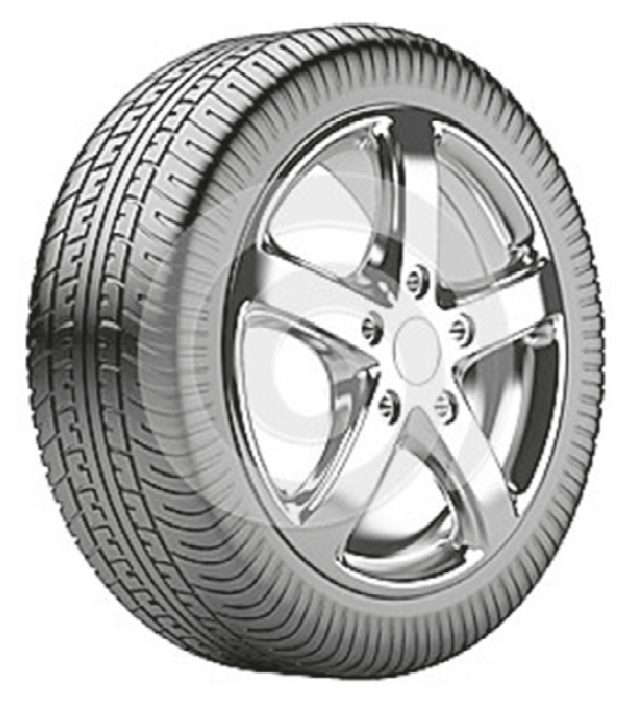
\includegraphics[width=4cm]{Organisation_gestion_donnees/Images/D6_ex_roue}
   \end{center}
   \begin{enumerate}
      \item Calculer la circonférence de cette roue en cm (arrondie au millimètre).
      \item La voiture roule à 110 km/h.
         \begin{enumerate}
            \item Calculer le nombre de tours par seconde que fait la roue (au tour près).
            \item La caméra utilisée a une vitesse de défilement de 24 images par seconde. \\
               Combien de tours aura fait le pneu de la voiture entre deux images ?
         \end{enumerate}
      \item À quelle vitesse, en km/h, devrait rouler la voiture pour que, en regardant le film, on ait l’impression que ses roues ne tournent pas ?
   \end{enumerate}
\end{exercice}

\begin{corrige}
\ \\ [-5mm]
\begin{enumerate}
   \item On a $\pi\times\text{diamètre} =54\,\pi\text{ cm} \approx169,646\text{ cm}$. {\blue La circonférence de la roue vaut environ 169,6 cm.}
   \item
      \begin{enumerate}
         \item La voiture parcourt :
            {\hautab{0.8}
            \begin{tabular}[t]{rl}
               110 km & en une heure ; \\
               11\,000\,000 cm & en 3\,600 secondes ; \\ [1mm]
               $\dfrac{11\,000\,000}{3\,600}\text{ cm} =\dfrac{27\,500}{9}\text{ cm}$ & en une seconde. \\
            \end{tabular}} \\
            Or, le périmètre de la roue fait 54$\pi$ cm donc en une seconde, on a $\dfrac{\dfrac{27\,500}{9}}{54\pi}\text{ tours} \approx18,01\text{ tours}$. \\
            {\blue La roue fait environ 18 tours par seconde.}
         \item En une seconde, la caméra fait 24 images et la roue 18 tours, donc entre deux images la roue fait \\
            $\dfrac{18}{24}$ tour = 0,75 tour. {\blue Le pneu aura fait 0,75 tour entre deux images.} \smallskip
      \end{enumerate}
   \setcounter{enumi}{1}
   \item Le nombre de tours est proportionnel à la vitesse, pour s'en convaincre, on peut d'écrire la formule du nombre de tours $T$ en fonction de la vitesse $v$ en km/h : \\ [1mm]
      $T =\dfrac{\dfrac{\text{vitesse en m/s}}{\text{périmètre en m}}}{\text{vitesse de défilement en images/s}} =\dfrac{\dfrac{\dfrac{100\,000\,v}{3\,600}}{54\pi}}{24} =\dfrac{100\,000\,v}{3\,600\times54\pi\times24} \approx 0,0068\,v$. \\ [2mm] 
      La roue semble ne pas tourner lorsqu'elle fait un cinquième de tour complet puisque, dans l'énoncé, il est précisé que la roue possède cinq rayons (on considère qu'elle contient cinq rayons identiques et que de plus, les portions entre deux rayons sont aussi identiques, ce qui semble être un implicite de l'énoncé). \\
      On sait d'après la question précédente qu'une vitesse de 110 km/h correspond à 0,75 tour entre \\ [1mm] deux images, donc pour avoir 0,2 tour, on effectue le calcul $\dfrac{110\times0,2}{0,75} \approx29,3$. \\
      {\blue La roue semble immobile à une vitesse d'environ 29 km/h ou tout multiple de 29 km/h. cohérent avec la réalité.}
   \end{enumerate}
\end{corrige}

\bigskip


\begin{exercice}[CRPE 2008 G2] %%%%%%%%%%%%%%%
   Deux robots, Arthur et Boz, sont placés aux deux extrémités d'une piste rectiligne de 300 mètres de long qui relie un point A à un point B. Arthur est placé au point A et Boz au point B. \\
   On les fait partir l'un vers l'autre à 9 heures précises. Arthur se déplace à la vitesse constante de 6 km/h et Boz à la vitesse constante de 24 km/h.
   \begin{enumerate}
      \item Exprimer ces deux vitesses en mètre par minute.
      \item On veut déterminer l'heure de rencontre des deux robots.
      \begin{enumerate}
         \item Représenter dans un même repère les déplacements des deux robots.
         \item Par lecture graphique, estimer l'heure de la rencontre.
      \end{enumerate}
      \item Déterminer par le calcul, l'heure de rencontre des deux robots.
   \end{enumerate}
\end{exercice}

\begin{corrige} 
\ \\ [-5mm]
\begin{enumerate}
   \item Arthur parcourt 6 kilomètres en 1 heure, soit 6 000 mètres en 60 minutes, ou encore 100 mètres en 1 minute. \\
      {\blue Arthur avance à une vitesse de 100 m/min.} \\
      Boz parcourt 24 kilomètres en 1 heure, soit 24 000 mètres en 60 minutes, ou encore 400 mètres en 1 minute. \\
      {\blue Boz avance à une vitesse de 400 m/min.}
   \item 
      \begin{enumerate}
         \item On note O, origine du repère, l'endroit où se trouve Arthur au départ, à 9 heures.
            \begin{itemize}
               \item Sur l'axe des abscisses, on représente la distance des robots au point O. À 9 heures, Arthur est en O alors que Boz est à 300 mètres du point O. On choisit (par exemple) une échelle de 1 cm pour 20 mètres en abscisse. 
               \item Sur l'axe des ordonnées, on représente le temps écoulé, en minutes, à partir de 9 h 00. Pour parcourir les 300 mètres, le robot le plus lent : Arthur, mettra 3 minutes. On choisit 1 cm pour 30 secondes en ordonnée.
               \item Courbe d'Arthur : sa vitesse est uniforme, sa courbe est donc une droite passant par l'origine et par le point de coordonnées (100;1) puisqu'il a une vitesse de 100 m/min.
               \item Courbe de Boz : sa vitesse est uniforme également, sa courbe est donc une droite passant par son point de départ représenté en (300;0). Sa vitesse est de 400 m/min, il aura donc parcouru 200 mètres en 0,5 minute, graphiquement, cela correspond au point de coordonnées (100;0,5).
            \end{itemize}
            {\psset{unit=0.9cm}
            \begin{pspicture}(-0.9,-1.5)(16,7.7)         
               \psgrid[subgriddiv=10, gridlabels=0, gridwidth=0.4pt, subgridwidth=0.4pt,gridcolor=brown!80,subgridcolor=brown!40](-1,-1)(16,7)
               \psaxes[dx=5,Dx=100,dy=2]{->}(0,0)(16,7)
               \rput(14,-1){distance en mètres de O}
               \rput(2.7,6.5){minutes écoulées depuis 9 h 00}
               \psline[showpoints=true,linecolor=B2](0,0)(5,2)(10,4)(15,6)
               \psline[showpoints=true,linecolor=A1](15,0)(10,0.5)(5,1)(0,1.5)
               \rput(14,0.8){\textcolor{A1}{déplacement de Boz}}
               \rput(14,6.5){\textcolor{B2}{déplacement d'Arthur}}
               \psline[linestyle=dashed](3,1.2)(3,0)
               \psline[showpoints=true,linestyle=dashed]{*->}(3,1.2)(0,1.2)
               \rput(-0.5,1.2){\fbox{0,6}}
            \end{pspicture}}
         \item Graphiquement, il suffit de trouver le point d'intersection des courbes de déplacement des deux robots, puis de lire son ordonnée : on trouve 0,6 minutes, soit 36 secondes. \\
            {\blue Les deux robots se rencontreront à 9 h 00 min 36 s.}
         \end{enumerate}
         \smallskip
      \setcounter{enumi}{2}
      \item On sait que $v=\dfrac{d}{t}$, donc $d=v\times t$ où on exprimera $v$ en mètre par minute, $d$ en mètre et $t$ en minute. \\ [1mm]
         Pour Arthur, on a $d_A =100\,t_A$ ; pour Boz, on a $d_B=400\,t_B$. \\
         Au point de rencontre, le même temps se sera écoulé, donc $t=t_A=t_B$ ; \\   
         de plus, la distance totale parcourue par les deux robots sera de 300 mètres, soit : \\
         $d_A+d_B=300 \iff 100t+400t =300$ \\
         \hspace*{2.1cm} $\iff 500t=300$ \\
         \hspace*{2.1cm} $\iff t=\dfrac{300}{500} =0,6$. \\ [1mm]
         On obtient un temps écoulé de 0,6 minute, soit $0,6\times\us{60} = \us{36}$. \\ [1mm]
         {\blue Les deux robots se rencontreront à 9 h 00 min 36 s.}
   \end{enumerate}
\end{corrige}

\pagebreak


\begin{exercice}[CRPE 2019 G2]
   Répondre aux quatre questions suivantes en utilisant les trois documents ci-après.
   \begin{enumerate}
      \item Un véhicule a parcouru le tronçon du tunnel de Noailles et la vitesse moyenne calculée est de 123 km/h.\\
         Quelle seras la vitesse retenue ?
      \item Un autre véhicule a parcouru la distance entre les deux points d’enregistrement en 4 minutes. \\
         Quelle sera la vitesse retenue ?
      \item Sur une contravention reçue suite à un excès de vitesse sur ce tronçon, la vitesse retenue est 114 km/h. \\
         Quelle était la vitesse moyenne calculée par l’ordinateur pour ce véhicule ?
      \item La plaque d’immatriculation d’un véhicule est enregistrée à 9 h 17 min 56 s devant le premier radar, puis à \\
         9 h 22 min 07 s devant le second radar. \\
         Le conducteur de ce véhicule sera-t-il sanctionné par une contravention ?
   \end{enumerate}
   \vfill
   \begin{center}
      {\bf Document 1 : Le radar tronçon du tunnel de Noailles} \\ [1mm]
      \fbox{
         \begin{minipage}{11cm}
            \it La portion de l’autoroute A20 entre Toulouse et Paris est équipée d’un radar-tronçon sur une distance de \ukm{5,1} à proximité du tunnel de Noaillles. \\
            La vitesse est limitée à 70 km/h lors de travaux de réfection du tunnel.
         \end{minipage}}
      \vfill
      {\bf Document 2 : Principe de fonctionnement d'un radar-tronçon}
      \begin{center}
         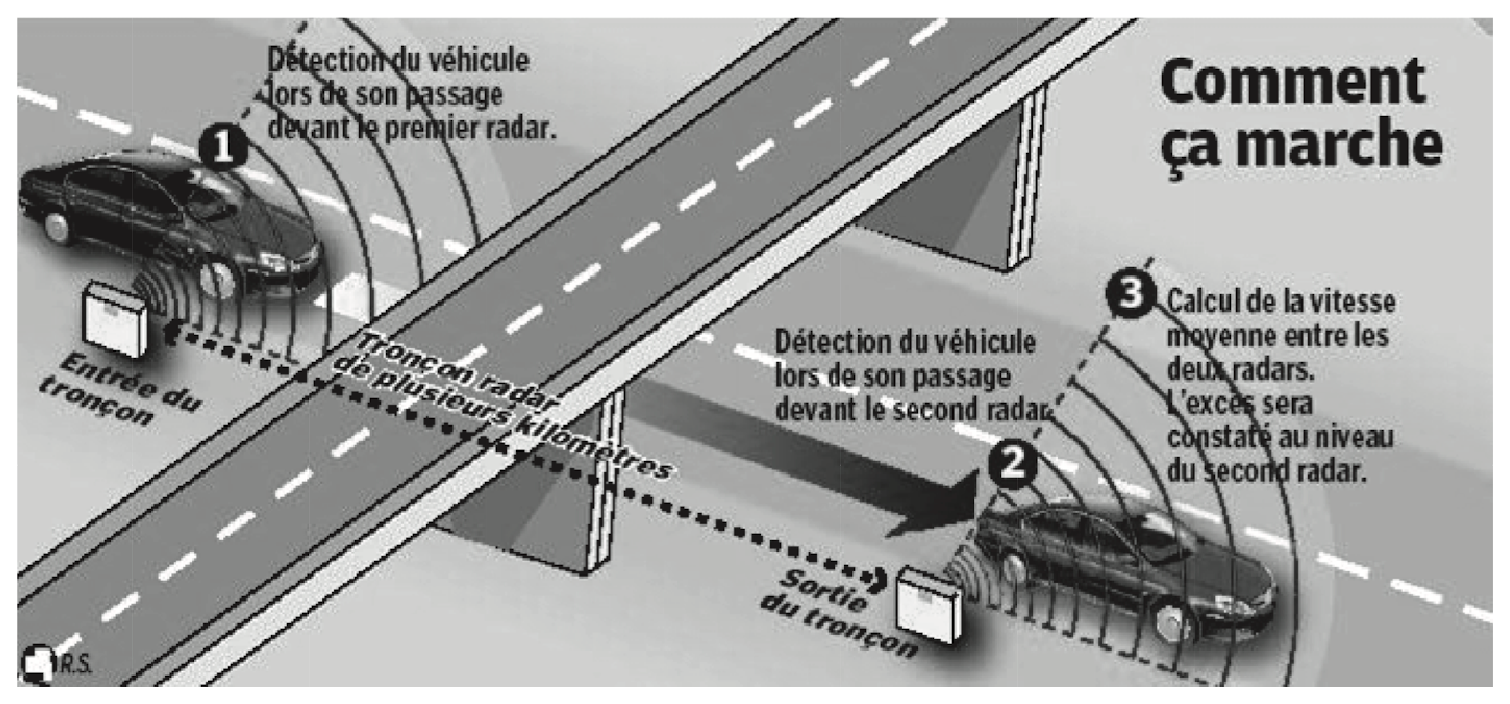
\includegraphics[width=15cm]{Organisation_gestion_donnees/Images/D6_ex_radar}
       \end{center}
       \vfill
      {\bf Document 3 : Calcul de la vitesse retenue pour la contravention} \\ [1mm]
      \fbox{
      \begin{minipage}{11cm}
         \it Un ordinateur calcule la vitesse moyenne de la voiture sur le tronçon puis détermine la vitesse retenue afin de prendre en compte les erreurs de précision du radar. \\
      Si la vitesse retenue est au-dessus de la vitesse limite, l’automobiliste reçoit une contravention.
      \end{minipage}} \\ [5mm]
      \begin{tabular}{|C{4}|C{4}|C{4}|}
         \hline
         Vitesse moyenne calculée par l'ordinateur & inférieure ou égale à 100~km/h & supérieure à 100~km/h \\
         \hline
         Vitesse retenue & On enlève 5 km/h à la vitesse moyenne calculée & On diminue la vitesse moyenne calculée de 5\,\% \\
         \hline 
      \end{tabular}
   \end{center}
\end{exercice}

\begin{corrige}
\ \\ [-5mm]
   \begin{enumerate}
      \item D'après le document 3, étant donnée la vitesse moyenne calculée supérieure à 100 km/h, il faut diminuer la vitesse de 5\,\%, soit appliquer un coefficient multiplicateur de $1-\dfrac{5}{100} =0,95$. \\ [1mm]
         Or, $123\times0,95 =116,85$. Donc, {\blue La vitesse retenue est de 116,85 km/h}.
      \item L'automobiliste parcourt \ukm{5,1} (document 1) en \umin{4}. \\ [1mm]
         On a $v =\dfrac{d}{t} =\dfrac{\ukm{5,1}}{\umin{4}}$ \\ [2mm]
         \hspace*{17mm} $=\dfrac{\ukm{5,1}}{\dfrac{4}{60}\uh{}}$ \\ [1mm]
         \hspace*{17mm} $=5,1\times\dfrac{60}{4}\,\ukm{}/\uh{}$ \\ [1mm]
         \hspace*{17mm} $=76,5\,\ukm{}/\uh{}$. \\ [1mm]
         D'après le document 3, étant donnée la vitesse moyenne calculée inférieure à 100 km/h, il faut diminuer la vitesse de 5 km/h, soit 76,5 km/h $-$ 5 km/h = 71,5 km/h. \\
         Conclusion : {\blue la vitesse retenue est de 71,5 km/h}.
      \item À une vitesse retenue de 114 km/h, la vitesse calculée était nécessairement supérieure, donc supérieure à 100 km/h, ce qui signifie qu'une réduction de 5\,\% a été appliquée à la vitesse calculée. \\ [1mm]
         Soit $v$ la vitesse calculée, on a alors $v\times0,95 =114\,\ukm{}/\uh{} \iff v =\dfrac{114\,\ukm{}/\uh{}}{0,95} =120\ukm{}/\uh{}$. \\
         {\blue La vitesse moyenne calculée était de 120 km/h}.
      \item Entre 9 h 17 min 56 s et 9 h 22 min 07, il s'est écoulé 4 min 11 s, soit \us{251}. \\
         Il a donc parcouru \ukm{5,1} en \us{251}. \\
         En \uh{1}, soit \us{3600}, il aurait donc parcouru $\dfrac{\ukm{5,1}\times\us{3600}}{\us{251}} \approx\ukm{73,15}$, d'où une vitesse de 73,15 km/h environ. \\
         La correction appliquée est un retrait de 5 km/h, soit 68,15 km/h. \\
         La vitesse étant limitée à 70 km/h, d'après le document 1, {\blue le conducteur ne sera pas verbalisé}.
   \end{enumerate}
\end{corrige}
   
\pagebreak  
 

\begin{exercice}[CRPE 2018 G3]
Au 1\up{er} janvier 2018, le Jamaïcain Usain Bolt détient le record du monde du 200 mètres en 19,19 secondes.
\begin{enumerate}
   \item Déterminer sa vitesse moyenne en km/h. Arrondir au dixième.
   \item À cette vitesse-là, combien mettrait-il de temps pour effectuer un marathon dont la longueur est de 42,195 km? On donnera la réponse en heures, minutes et secondes, arrondie à la seconde près.
   \item Le précédent record du monde du 200 mètres était détenu par l’américain Michael Johnson, \og La locomotive de Wako \fg», avec un temps de 19,32 secondes aux Jeux Olympiques d’Atlanta en 1996. \\
   De quel pourcentage Usain Bolt a-t-il réduit le temps du record du monde du 200 mètres ?
\end{enumerate}
\end{exercice}

\begin{corrige}
\ \\ [-5mm]
   \begin{enumerate}
      \item $\text{vitesse} =\dfrac{\text{distance}}{\text{temps}}$ donc : \\ [1mm]
         $v =\dfrac{200\text{ m}}{19,19\text{ s}} =\dfrac{0,2\text{ km}}{\dfrac{19,19}{3\,600\text{ h}}} \approx37,52\text{ km/h}.$ \\ [1mm] 
        {\blue La vitesse d'Usain Bolt sur 200 m est d'environ 37,5 km/h.} \\ [1mm]
      \item $v =\dfrac{d}{t} \iff t =\dfrac{d}{v} =\dfrac{42,195\text{ km}}{37,52\text{ km/h}} \approx1,125\text{ h}$. \\ [1mm] 
         Or, 1,125 h = 1 h + 0,125 h \\
         \hspace*{1.54cm} = 1 h + 0,125$\times$60 min \\
         \hspace*{1.54cm} = 1 h + 7,5 min \\
         \hspace*{1.54cm} = 1h + 7 min + 30 s. \\
         {\blue À cette allure, Usain Bolt mettrait 1 h 7 min 30 s pour arriver au bout d'un marathon.} \\ [1mm]
      \item $p =\dfrac{t_{\text{Bolt}}-t_{\text{Johnson}}}{t_{\text{Johnson}}}\times100$ \\ [1mm]
          \hspace*{6.5mm} $=\dfrac{19,19\text{ s}-19,32\text{ s}}{19,32\text{ s}}\times100 \approx-0,67$. \\ [1mm]
         {\blue Usain Bolt a réduit le temps de Michael Johnson de 0,67\,\%.}
   \end{enumerate} 
\end{corrige}


\bigskip


\begin{exercice}[CRPE 2017 G1-G3 et 2018 G1-G3] %%% 9
   Indiquer si les affirmations suivantes sont vraies ou fausses en justifiant la réponse. Une réponse exacte, mais non justifiée, ne rapporte aucun point. Une réponse fausse n’enlève pas de point.
   \begin{enumerate}
      \item On réduit respectivement la largeur et la longueur d’un rectangle de 20\,\% et 10\,\%. \\
         {\bf Affirmation :} \og L’aire du rectangle ainsi obtenu a diminué de 28\,\%. \fg
      \item Un rectangle a une largeur et une longueur qui mesurent respectivement 6 cm et 9 cm. On réduit la largeur de 20\,\% et la longueur de 10\,\%. \\
         {\bf Affirmation :} \og Le périmètre du rectangle ainsi obtenu a diminué de 15\,\%. \fg
      \item {\bf Affirmation :} durant les soldes si on baisse le prix d’un article de 30 \,\% puis de 20\,\%, alors le prix de l’article a baissé de 50\,\%.
      \item Un prix subit une baisse de 30\,\% puis le nouveau prix subit une hausse de 50\,\%. \\
         {\bf Affirmation :} le prix final est 5\,\% plus élevé que le prix initial.
      \item {\bf Affirmation :} si des prix augmentent de 5\,\% par an, ils auront plus que doublé en 15 ans.
      \item Arthur a acheté un article bénéficiant d’une réduction de 30\,\% et a ainsi économisé 48 \euro. \\
         {\bf Affirmation :} Au final, il a payé 112 \euro{} pour cet article.
   \end{enumerate}
\end{exercice}

\begin{corrige}
\ \\ [-5mm]
   \begin{enumerate}
      \item On note $\mathcal{A}_i$ l'aire initiale et $\mathcal{A}_f$ l'aire finale après transformation. Soit $\ell$ et $L$ respectivement la largeur et la longueur d'un rectangle. L'aire initiale du rectangle est $\mathcal{A}_i =\ell L$. \\
         Une réduction de 20\% correspond à un coefficient multiplicateur de $1-\dfrac{20}{100} =0,8$ et une réduction de 10\% correspond à un coefficient multiplicateur de $1-\dfrac{10}{100} =0,9$. \\
          D'où $\mathcal{A}_f =0,8\ell\times0,9L =0,72\ell L =\left(1-\dfrac{28}{100}\right)\mathcal{A}_i$ ce qui correspond à une diminution de 28\%. \\
         {\blue L'affirmation est vraie.}
      \item On note $P_i$ le périmètre initial et $P_f$ le périmètre final après transformation. En reprenant les coefficients multiplicateurs de l'item précédent, on trouve : \\
         $P_i =2(6\text{ cm}+9\text{ cm}) =30$ cm et $P_f =2(0,8\times6\text{ cm}+0,9\times9\text{ cm}) =25,8$ cm. \\
         Or, une diminution de 15\% donnerait un périmètre $P_f =0,85\times29\text{ cm} =24,65$ cm ce qui n'est pas le cas. \\
          {\blue L'affirmation est fausse.}
       \item Un baisse de 30\,\% suivie d'une baisse de 20\,\% correspond à un coefficient multiplicateur de \\ [1mm]
          $\left(1-\dfrac{30}{100}\right)\times\left(1-\dfrac{20}{100}\right) =0,7\times0,8 =0,56 =1-\dfrac{44}{100}$. Soit une baisse de 44\,\%. \\ [1mm]
          {\blue L'affirmation est fausse.}
       \item Une baisse de 30\,\% correspond à un coefficient multiplicateur de $1-\dfrac{30}{100} =0,7$ et une hausse de 50\,\% correspond à un coefficient de $1+\dfrac{50}{100} =1,5$. Le coefficient résultant de ces deux variations vaut $0,7\times1,5 =1,05 =1+\dfrac{5}{100}$ ce qui correspond à une augmentation de 5\,\%. \\ [1mm]
         {\blue L'affirmation est vraie.}
      \item Une augmentation de 5\,\% correspond à un coefficient multiplicateur de $1+\dfrac{5}{100} =1,05$. \\
         Au bout de 15 ans, le coefficient sera de $1,05^{15} \approx2,08 >2$. \\ [1mm]
         {\blue L'affirmation est vraie.}
      \item Soit $x$ le prix initial, $x\times\dfrac{30}{100} =48 \iff x =160$. Le prix initial est de 160 \euro{}, auquel on enlève la réduction \\ [1mm]
   de 48 \euro{} ce qui donne bien 112 \euro. \\ [1mm]
       {\blue L'affirmation est vraie.} \\ [3mm]
   \end{enumerate}
\end{corrige}

\bigskip


\begin{exercice}[Histoires de ratios]
   Les trois questions suivantes sont indépendantes.
   \begin{enumerate}
      \item On considère le tableau suivant représentant le nombre de matchs gagnés et perdu en rugby, judo et handball durant une rencontre inter-clubs. \medskip
         \begin{center}
            {\hautab{1.2}
            \begin{cltableau}{0.5\linewidth}{3}
               \hline
               Sport & matchs gagnés & matchs perdus \\
               \hline
               Rugby & 9 & 6 \\
               \hline
               Judo & 12 & 8 \\
               \hline
               Handball & 10 & 5 \\
               \hline
            \end{cltableau}}
         \end{center}
         \begin{enumerate}
           \item Quels sports ont un ratio équivalent gains-pertes ?
            \item Pour le handball, quel est le ratio gains-matchs joués ? Quelle est la fraction de matchs gagnés ? Quel est le pourcentage de matchs gagnés ? \\ [-10mm]
         \end{enumerate}
      \item Deux amis ont joué au loto et leur mise s'est faite selon le ratio 3 : 5. Ils gagnent \ueuro{64}. \\
         Quelle est la somme d'argent qui revient à chacun d'eux ?
      \item Adam va fêter ses 10 ans. Avant son anniversaire, il essaie une nouvelle recette de cocktail sans alcool, pour laquelle il faut 2 verres de jus d'orange pour 3 verres de jus d'ananas et 4 verres de jus de pomme. \\
         Cette recette lui plaît. Pour tous ses amis, il veut préparer \ul{45} de cocktail. \\
         Combien de litres de chaque ingrédient doit-il acheter ?
   \end{enumerate}
\end{exercice}

\begin{corrige}
\ \\ [-5mm]
   \begin{enumerate}
      \item 
         \begin{enumerate}
            \item Pour le rugby, le ratio gains - pertes est de 9 : 6, ou encore 3 : 2. \\
               Pour le judo, le ratio gains - pertes est de 12 : 8, soit 3 : 2. \\
               Pour le handball, le ratio gains - pertes de 10 : 5, ou 2 : 1. \\
               Conclusion : {\blue le rugby et le judo ont le même ratio gains - pertes}.
            \item Pour le handball, le ratio gains - matchs joués est de 10 : 15 équivalent à {\blue 2 : 3}. \\ [1mm]
               La fraction de matchs gagnés est de $\dfrac{10}{15} = \blue \dfrac23$. \\ [1.5mm]
               Le pourcentage de matchs gagnés est de $\dfrac{10}{15}\times100 \approx {\blue 67\,\%}$. \smallskip
         \end{enumerate}   
      \setcounter{enumi}{1}
      \item Le ratio 3 : 5 signifie que lorsqu'un joueur gagne \ueuro{3}, l'autre gagne \ueuro{5} pour une somme de \ueuro{8}. \\
         S'ils gagnent \ueuro{64}, c'est à dire 8 fois plus, {\blue l'un gagnera \ueuro{24} et l'autre \ueuro{40}}. \\
      \item Le jus d'orange, d'ananas et de pomme sont dans le ratio 2 : 3 : 4. Donc, pour \ul{2} de jus d'orange, il faut \ul{3} de jus d'ananas et \ul{4} de jus de pomme ce qui donne \ul{9} de cocktail. \\
         Pour \ul{45}, soit 5 fois plus, il faut {\blue \ul{10} de jus d'orange, \ul{15} de jus d'ananas et \ul{20} de jus de pomme}.
   \end{enumerate}
\end{corrige}


% \begin{exercice}[À vos papyrus !] %%%%%%%%%%%%%%
%   Faisons un voyage temporel de 3 500 années en arrière. Nous nous retrouvons au temps de l’Egypte antique, et plus précisément dans le nouvel empire. {\it Ahmès}, le scribe, vient juste d’écrire le Papyrus Rhind, un document comportant près de 90 problèmes mathématiques résolus en tous genre (arithmétique, géométrie etc.). \\
%   Voici une transcription du problème 24 du Papyrus Rhind :
%\begin{center}
%\fbox{
%\begin{minipage}{9cm}
%   Une quantité son $\overline{7}$ lui est ajouté. Elle devient 19. \\
%   Quelle est cette quantité ? \\
%   \begin{tabular}{C{1}p{1.5cm}p{1.5cm}}
%      & 1 \slash & 7 \\
%      & $\overline{7}$ \slash & 1 \\
%      & \bm{Total} & \bm{8} \\
%      & 1 & 8 \\
%      & 2 \slash & 16 \\
%      & $\overline{2}$ & 4 \\
%      & $\overline{4}$ \slash & 2 \\
%      & $\overline{8}$ \slash & 1 \\
%      & \bm{2 \, $\overline{4}$ \, $\overline{8}$} & \bm{19} \\
%      & 1 \slash & 2 \, $\overline{4}$ \, $\overline{8}$ \\
%      & 2 \slash & 4 \, $\overline{2}$ \, $\overline{4}$ \\
%      & 4 \slash & 9 \,  $\overline{2}$ \\
%      & 7 & 16 \, $\overline{2}$ \, $\overline{8}$ \\
%      & $\overline{7}$ & 2 \, $\overline{4}$ \, $\overline{8}$ \\
%      & Total & 19 \\
%   \end{tabular} \\
%   {\bm Réponse : 16 \, $\overline{2}$ \, $\overline{8}$}
%\end{minipage}}
%\end{center}
%\begin{enumerate}
%   \item Résoudre le problème d'une manière algébrique.
%   \item À quoi servent les barres obliques à côté de certains nombres et la barre au dessus d'autres nombres ?
%   \item Expliquer les étapes du scribes.   
%   \item Pourquoi avoir choisi 7 comme nombre de départ ?
%   \item Quells sont les opérations et principes mathématiques présents dans les calculs ?
%   \item La méthode utilisée par le scribe s’appelle la méthode de la \og fausse position simple \fg. Qu’est-ce qui justifie cette appellation ?
%\end{enumerate}
%\end{center}
%\end{exercice}
%
%\begin{corrige}
%\begin{enumerate}
%   \item Soit $x$ le nombre recherché, il s'agit de résoudre l'équation : \\ [1mm]$x+\dfrac17x =19 \iff \dfrac87x=19 \iff x =19\times\dfrac78 \iff x = \dfrac{133}{8} =\dfrac{128+4+1}{8} \iff$ \bm{$x =16+\dfrac12+\dfrac18$}.
%   \smallskip
%   \item Les barres obliques sont des {\bm coches} qui permettent de cocher les nombres utilisés dans les additions. Les barres désignent des \bm{fractions de numérateur 1} et de dénominateur le nombre surligné.
%   \item On a les étapes suivantes : \\
%   \begin{tabular}{p{1.5cm}p{1.5cm}p{12cm}}
%      1 \slash & 7 &on choisit 7 comme nombre de départ \\
%      $\overline{7}$ \slash & 1 & son septième vaut 1 \\
%      Total & 8 & en choisissant 7 comme nombre de départ, le résultat est 8 qui est trop petit \\
%      1 & 8 & on cherche combien de fois 8 on peut mettre dans 19 : une fois la base 7 donne 8 \\
%      2 \slash & 16 & on duplique : 2 fois 8 la base 7 donne 16 \\
%      $\overline{2}$ & 4 & la moitié de la base 7 donne 4 \\
%      $\overline{4}$ \slash & 2 & la moitié de la moitié (le quart) de la base 7 donne 2 \\
%      $\overline{8}$ \slash & 1 & la moitié de la moitié de la moitié (le huitième) de la base 7 donne 1 \\
%      2 \, $\overline{4}$ \, $\overline{8}$ & 19 & 19 = 16 + 2 + 1, donc $8 \times\left(2 +\dfrac14+\dfrac18\right) =19$. \\
%      1 \slash & 2 \, $\overline{4}$ \, $\overline{8}$ & il reste à multiplier 7 par le coefficient multiplicateur $2 +\dfrac14+\dfrac18$ \\
%      2 \slash & 4 \, $\overline{2}$ \, $\overline{4}$ & 2 fois ce coefficient donne $4+\dfrac12+\dfrac14$ \\
%      4 \slash & 9 \,  $\overline{2}$ & on duplique de nouveau, ce qui donne $8+1+\dfrac12 =9+\dfrac12$ \\
%      7 & 16 \, $\overline{2}$ \, $\overline{8}$ & $7 =1+2+4$ donc $7\times\left(2 +\dfrac14+\dfrac18\right) =15+\dfrac22+\dfrac24+\dfrac18 =16+\dfrac12+\dfrac18$. \\
%      $\overline{7}$ & 2 \, $\overline{4}$ \, $\overline{8}$ & son septième vaut $2+\dfrac14+\dfrac18$ \\
%      Total & 19 & si on somme 7 et $\overline{7}$, cela donne bien $18+\dfrac12+\dfrac14+\dfrac28 =19$. \\
%   \end{tabular} \\
%   \bm{La réponse est $16+\dfrac12+\dfrac18$}.
%   \item 7 est choisi comme nombre de départ car son septième fait un, ce qui \bm{simplifie les calculs}.
%   \item Comme opérations, on utilise uniquement la \bm{duplication} (qui est une somme de deux nombres identiques) et la \bm{division par 2}. Le principe est celui de la \bm{proportionnalité}.
%   \item Il imagine une solution (la fausse position) à partir de laquelle il pose ses calculs. 
%\end{enumerate}
%\end{corrige}
